\chapter{Data visualization with \Visit}

\section{Introduction}
Visualization of \Vaango data is currently performed using \Visit. 
The \Visit package from LLNL is general purpose visualization software
that offers all of the usual capabilities for rendering scientific
data.  It is developed and maintained by LLNL staff, and its
interface to \Vaango data is supported by the \Uintah team. The latest
\Visit version that \Vaango has been tested on is \Visit 3.1.1.
The UDA reader plugin is currently incorporated directly into \Visit
and does not have to be installed separately.

You can install \Visit by downloading one of the pre-built executables from
\url{https://wci.llnl.gov/simulation/computer-codes/visit/executables}.
Alternatively, you can build your own version from source using instructions 
given in the \Visit web page.

\columnratio{0.7}
\globalcounter{figure}
%\setcolumnwidth{0.5\textwidth,0.3\textwidth}
\begin{paracol}{2}
  \section{Particle data visualization}
  To visualize particle information, run \Visit.  
  To open a UDA, select \Textsfc{Open File} from the \Textsfc{File} menu
  (Figure~\ref{fig:visit_2}). Browse into
  the UDA you want to load (Figure~\ref{fig:visit_3}) and select the \Textsfc{index.xml}
  file (Figure~\ref{fig:visit_4}). Then hit on \Textsfc{OK} and a list of timesteps should
  now appear on the gui (Figure~\ref{fig:visit_6}). 

  \switchcolumn

  \begin{figure}[htb!]
    \centering
    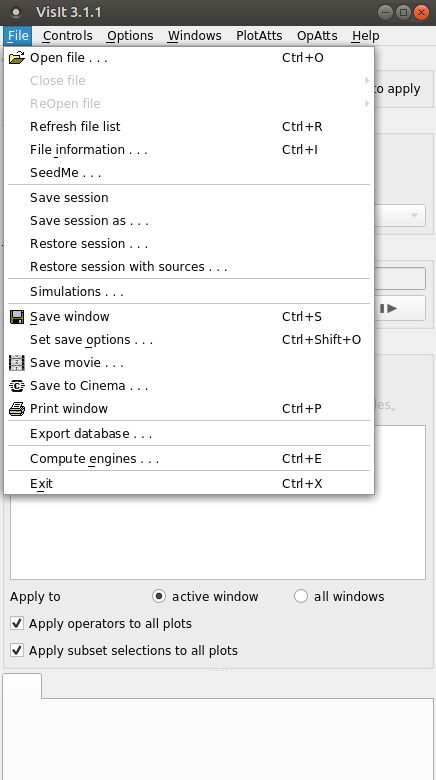
\includegraphics[width=0.9\columnwidth]{FIGS/visit/visit_2.png}
    \caption{\Visit control window.}
    \label{fig:visit_2}
  \end{figure}

  \switchcolumn
  \begin{figure}[htb!]
    \centering
    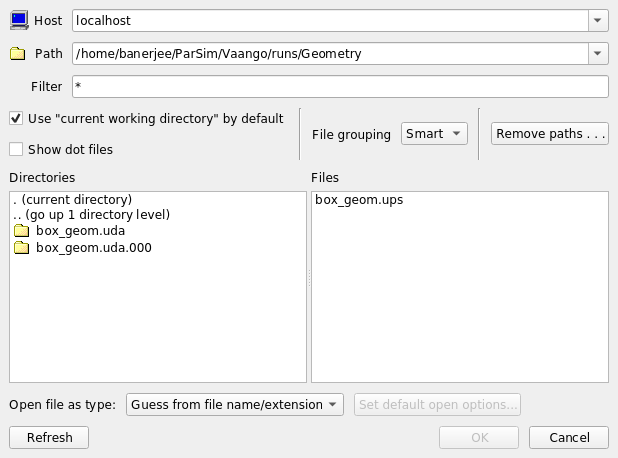
\includegraphics[width=0.5\columnwidth]{FIGS/visit/visit_3.png}
    \caption{\Visit file open dialog.}
    \label{fig:visit_3}
  \end{figure}

  \begin{figure}[htb!]
    \centering
    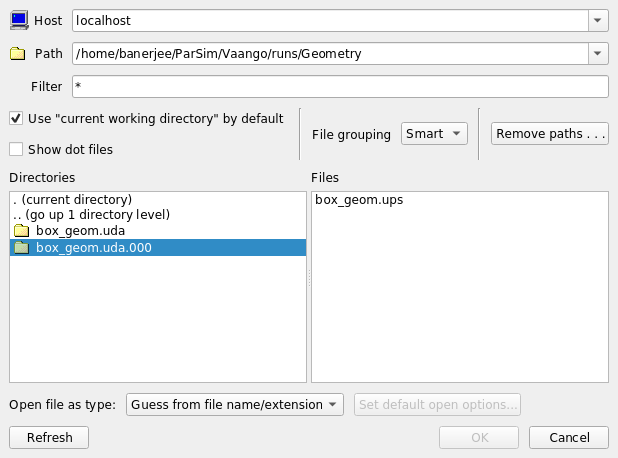
\includegraphics[width=0.5\columnwidth]{FIGS/visit/visit_4.png}
    \caption{Selecting a UDA to load.}
    \label{fig:visit_4}
  \end{figure}

  \switchcolumn
  \begin{figure}[htb!]
    \centering
    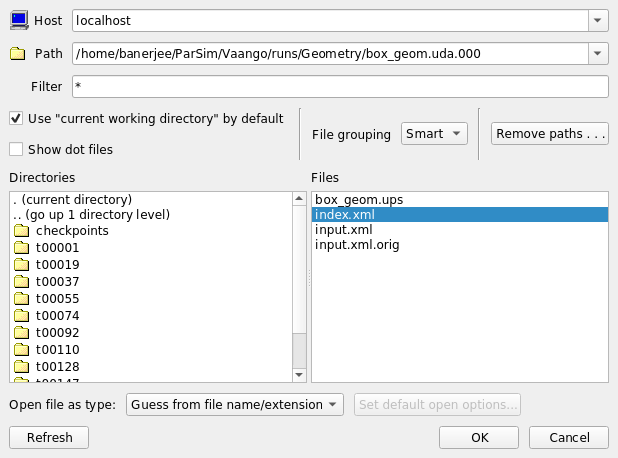
\includegraphics[width=\columnwidth]{FIGS/visit/visit_6.png}
    \caption{Selecting the index.xml file.}
    \label{fig:visit_6}
  \end{figure}

  \switchcolumn
  Now a window indicating an active source is created with an \Textsfc{Add}
  button.  Click on this button and select \Textsfc{Pseudocolor} and the
  particle variable \Textsfc{p.volume} (or any other quantity that is
  available in the UDA) as shown in Figure~\ref{fig:visit_10}.
  This allows you to plot \Textsfc{scalar} quantities that are associated
  with the \MPM particles.
  The variable to be plotted is highlighted in green.  Click on the \Textsfc{Draw}
  button (Figure~\ref{fig:visit_12}) to visualize the data.

  \begin{figure}[htb!]
    \centering
    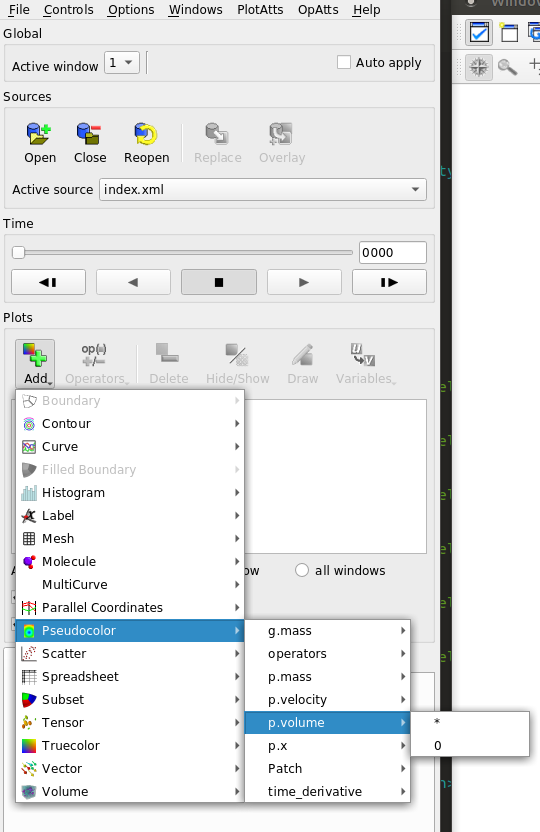
\includegraphics[width=0.5\columnwidth]{FIGS/visit/visit_10.png}
    \caption{Selecting the scalar particle variable to plot.}
    \label{fig:visit_10}
  \end{figure}

  \switchcolumn

  \begin{figure}[htb!]
    \centering
    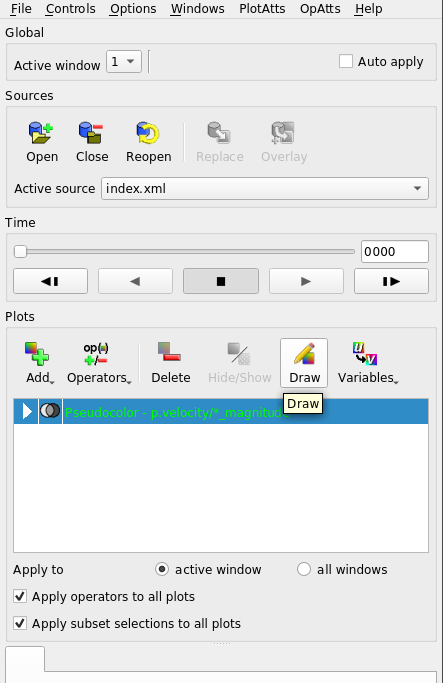
\includegraphics[width=0.9\columnwidth]{FIGS/visit/visit_12.png}
    \caption{Clicking on the \Textsfc{Draw} button.}
    \label{fig:visit_12}
  \end{figure}

  \switchcolumn

  A plot of the data shows up on the display window as seen in Figure~\ref{fig:visit_13}.
  \begin{figure}[htb!]
    \centering
    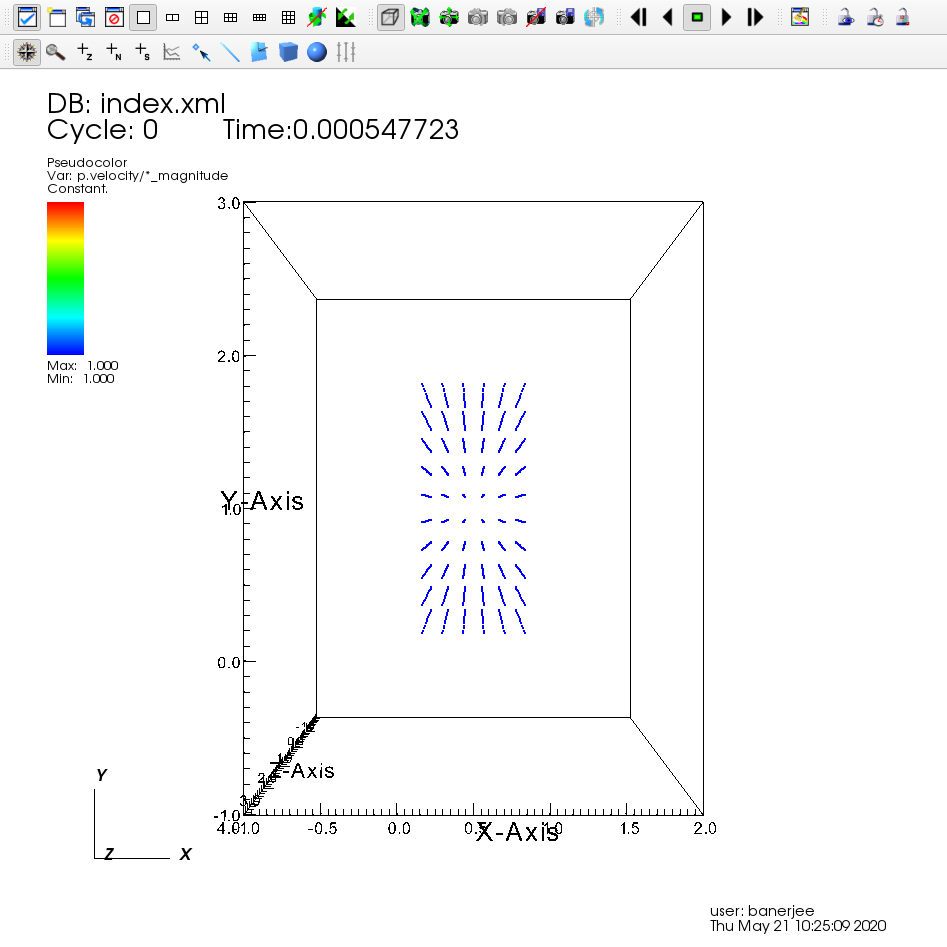
\includegraphics[width=0.4\columnwidth]{FIGS/visit/visit_13.png}
    \caption{Plot of the particle data in the UDA file.}
    \label{fig:visit_13}
  \end{figure}

  The particles are too small in this plot because they are represented as
  points.  We can increase the size by changing the particle type into spheres.
  To do that select \Textsfc{PlotAtts} as shown in Figure~\ref{fig:visit_18}.
  If you then choose the \Textsfc{Pseudocolor} item from the list, a window pops up 
  that allows you to modify the appearance of the particles (Figure~\ref{fig:visit_17}).
  Change the button for \Textsfc{Point Type} from \Textsfc{Point} tp \Textsfc{Sphere}
  (Figure~\ref{fig:visit_20}).
  
  \switchcolumn

  \begin{figure}[htb!]
    \centering
    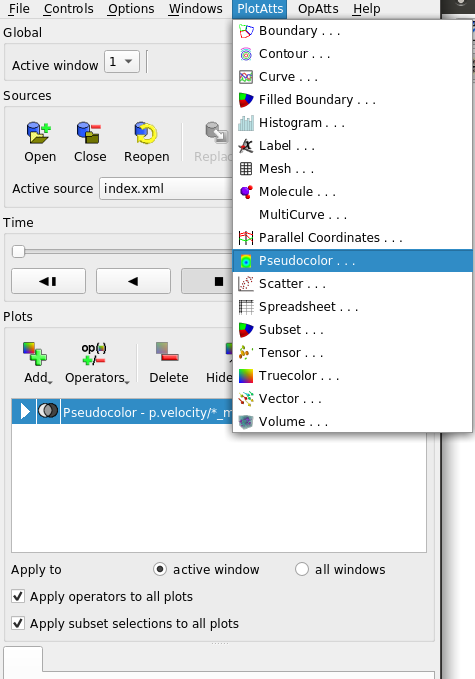
\includegraphics[width=\columnwidth]{FIGS/visit/visit_18.png}
    \caption{Selecting pseudocolor plot attributes.}
    \label{fig:visit_18}
  \end{figure}
  \begin{figure}[htb!]
    \centering
    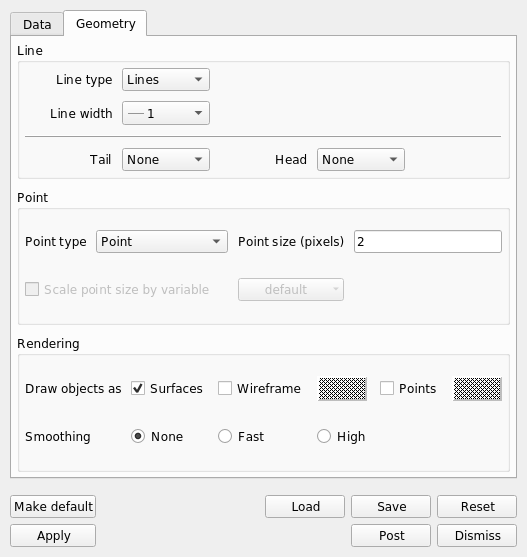
\includegraphics[width=\columnwidth]{FIGS/visit/visit_17.png}
    \caption{Changing the appearance of particles.}
    \label{fig:visit_17}
  \end{figure}

  \switchcolumn

  \begin{figure}[htb!]
    \centering
    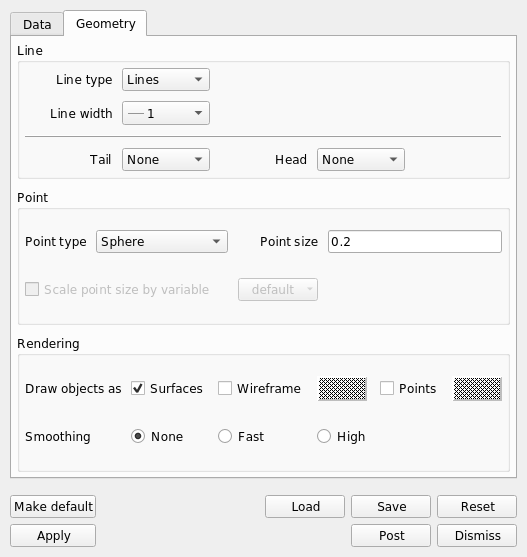
\includegraphics[width=0.5\columnwidth]{FIGS/visit/visit_20.png}
    \caption{Switching from point to sphere respresentation.}
    \label{fig:visit_20}
  \end{figure}

  \switchcolumn

  \begin{figure}[htb!]
    \centering
    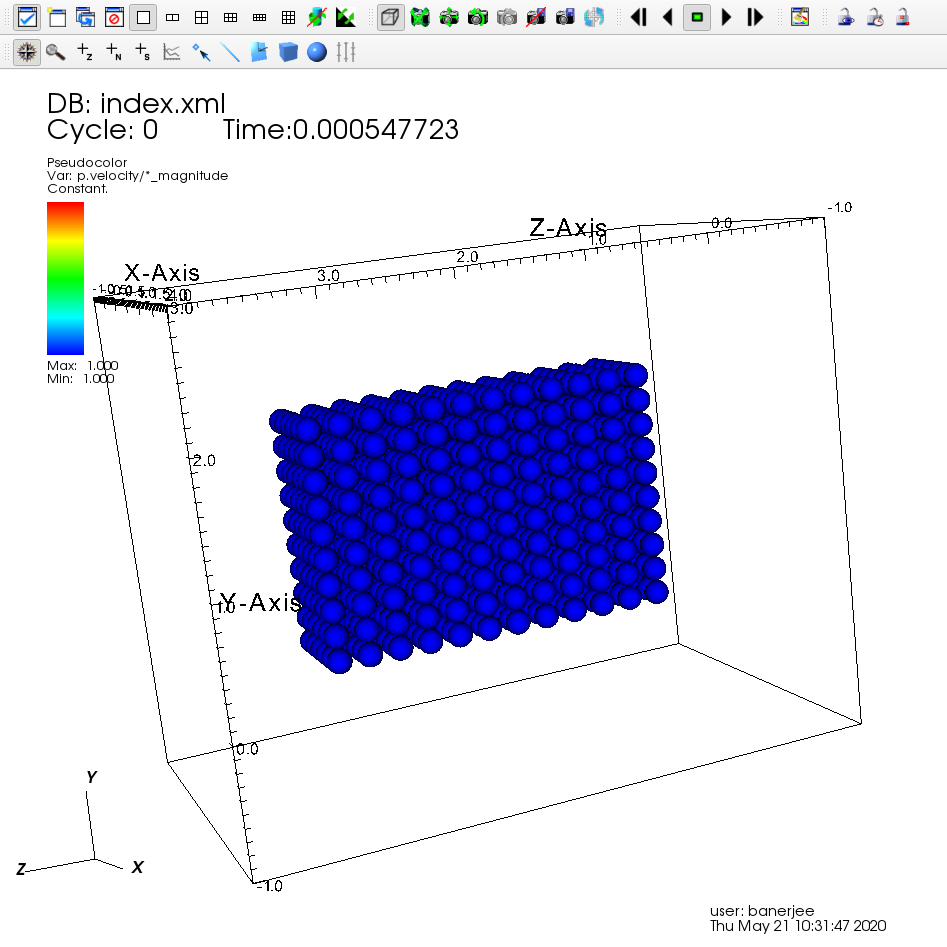
\includegraphics[width=\columnwidth]{FIGS/visit/visit_21.png}
    \caption{Particles drawn as spheres.}
    \label{fig:visit_21}
  \end{figure}

  \switchcolumn
  Figure~\ref{fig:visit_21} shows the updated view of the \MPM particles.
  However, the color is still too dark.  If you want a lighter color, you 
  will have to change the \Textsfc{color map} (Figure~\ref{fig:visit_23}.
  Select any one of the options that pops up when you select \Textsfc{Color table}
  and you will get a set of particles colored differently from the default
  as seen in Figure~\ref{fig:visit_24}.

  \switchcolumn
  \begin{figure}[htb!]
    \centering
    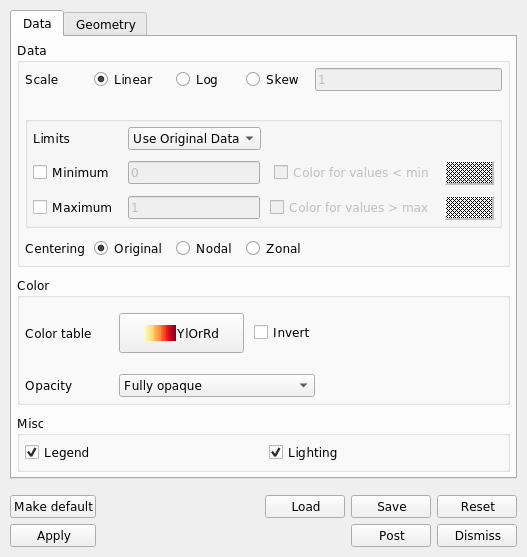
\includegraphics[width=\columnwidth]{FIGS/visit/visit_23.png}
    \caption{Changing the color map.}
    \label{fig:visit_23}
  \end{figure}

  \switchcolumn

  \begin{figure}[htb!]
    \centering
    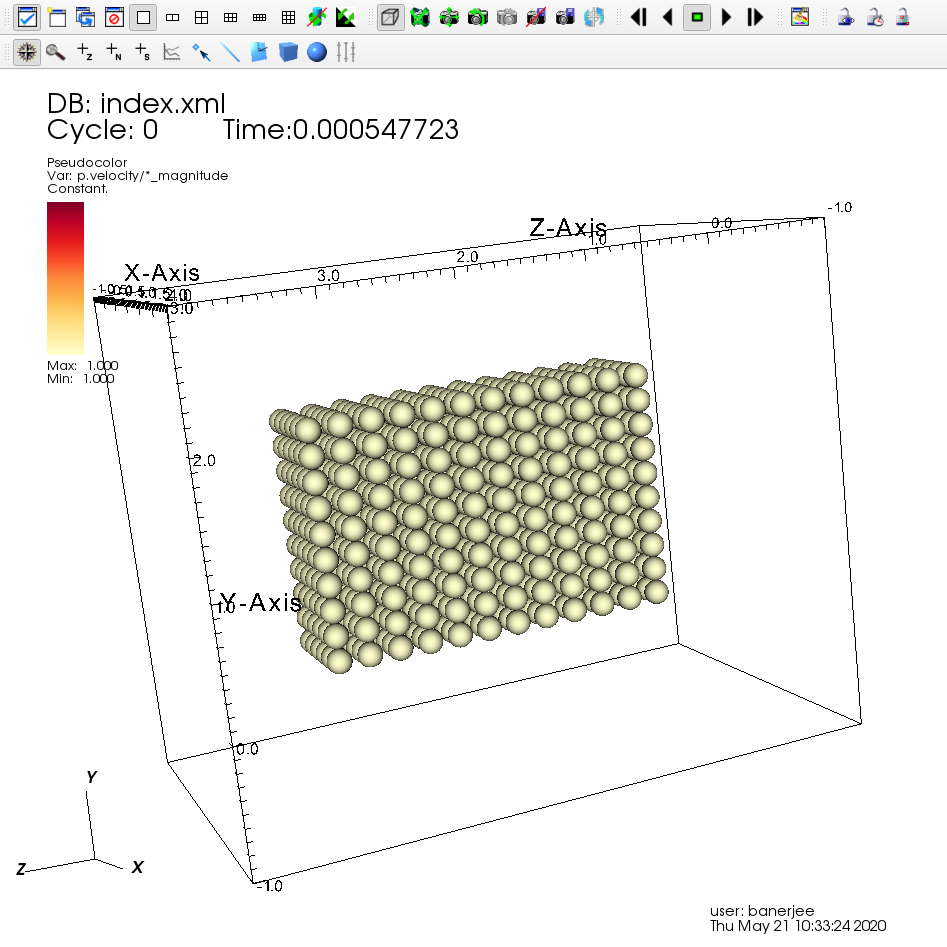
\includegraphics[width=0.7\columnwidth]{FIGS/visit/visit_24.png}
    \caption{Changing the appearance of particles.}
    \label{fig:visit_24}
  \end{figure}
  
\end{paracol}

\newpage
\begin{minipage}[t]{\textwidth}
  \begin{minipage}{0.6\textwidth}
  \vspace{-48pt}
  \section{Volumetric data plots}
  \Visit displays data as plots. A plot might render a specific variable
  or it might render the structure of the mesh. Figure~\ref{VisItPlots}
  illustrates this.
  Note that \Visit attempts to analyze the variables and associate them
  with the appropriate plots. As shown in Figure~\ref{VisItPlots}, only
  vector variables are available for the vector plot. The most commonly
  used plots for visualizing UDA's are Pseudocolor, Volume and the
  Vector plot. The Subset plot can be used to visualize the structure of
  patches in an AMR dataset.
  \end{minipage}
  \hspace{12pt}
  \begin{minipage}{0.35\textwidth}
    \centering
    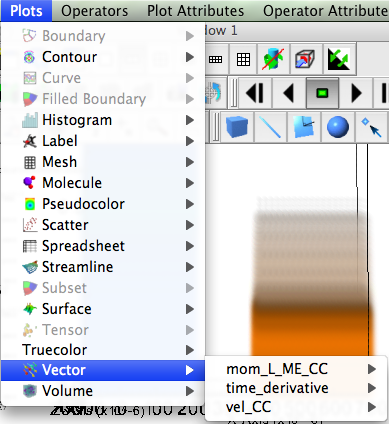
\includegraphics[width=\textwidth]{VisItPlots.png}
    \captionof{figure}{Various plots in \Visit}
    \label{VisItPlots}
  \end{minipage}
\end{minipage}

\begin{minipage}[t]{\textwidth}
  \begin{minipage}{0.6\textwidth}
  \vspace{-96pt}
  Once you have a plot, you change plot attributes by clicking on the
  PlotAtts menu and selecting the plot of you choice. Alternatively, you
  may double click on the plot itself in Active plots window. For
  example, if you have a Volume plot and you want to change its
  attributes, the window shown in Figure~\ref{VisItVolumeAtts} pops up.

  As seen in Figure~\ref{VisItVolumeAtts}, you can change the color map,
  opacity curve, rendering method, no. of samples, lighting options,
  etc. in this window.
  \end{minipage}
  \hspace{12pt}
  \begin{minipage}{0.35\textwidth}
  \centering
  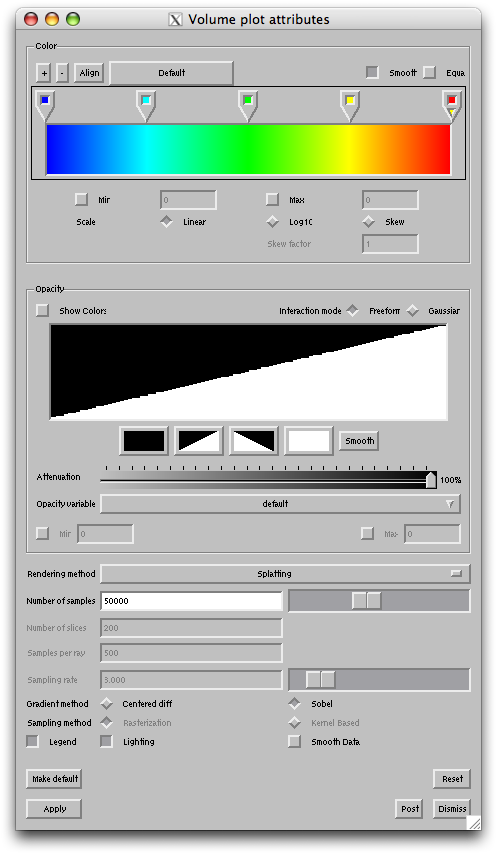
\includegraphics[width=0.8\textwidth]{VisItVolumeAtts.png}
  \captionof{figure}{Volume plot attributes in \Visit}
  \label{VisItVolumeAtts}
  \end{minipage}
\end{minipage}

\section{Operators}
\begin{wrapfigure}[3]{r}{.50\textwidth}
  \vspace{-20pt}
  \centering
  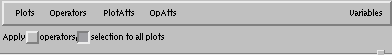
\includegraphics[width=.3\textwidth]{VisItApplyOperators.png}
  \vspace{-10pt}
  \caption{Unchecking "selection to all plots"}
  %\vspace{-10pt}
  \label{VisItApplyOperators}
\end{wrapfigure}

A wide variety of operators can be applied to the plots, as mentioned
earlier. These modify the incoming datasets in some way (eg., a slice
formats a 3D dataset into a 2D slice), which can then be
plotted. However, you will first need to select a plot and then only
you can apply an operator to it (though the order of operation is
opposite). An important thing to keep in mind is that when you select
an operator, by default it gets applied to all the plots in the Active
plots window. You will need to uncheck the Apply operators checkbox,
in case you just want to apply the operator to a single plot as shown
in Figure~\ref{VisItApplyOperators}.

The entire list of operators that \Visit supports can be seen by
clicking on the Operators menu. Also, once you have applied an
operator, you can change its attributes by clicking on the OpAtts menu
and then clicking on the desired operator.
Figures~\ref{VisItSelectPlot} and~\ref{VisItSelectOperator} illustrate
how you can apply a Slice operator to a Pseudocolor plot and then
change the operator attributes.  First, apply the Pseudocolor plot to
a desired variable, and then select the Slice operator from the
Operators menu.
\begin{figure}[htbp!]
  \begin{subfigure}[b]{0.5\textwidth}
    \centering 
    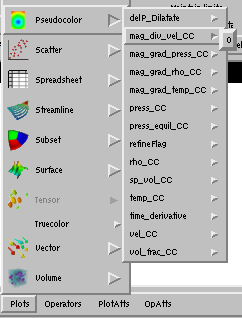
\includegraphics[height=0.2\textheight]{VisItSelectPlot.png}
    \caption{Applying the Pseudocolor plot to a variable}
    \label{VisItSelectPlot}
  \end{subfigure}
  \begin{subfigure}[b]{0.5\textwidth}
    \centering 
    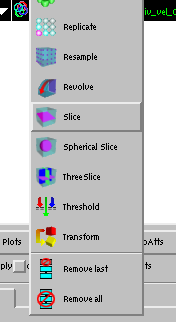
\includegraphics[height=0.2\textheight]{VisItSelectOperator.png}
    \caption{Applying an operator to a plot}
    \label{VisItSelectOperator}
  \end{subfigure}
  \caption{Pseudocolors and applying operators.}
  \label{ucf:fig1}
\end{figure}

At this point in time, you should have an ordering similar to that in
Figure~\ref{VisItOrderOperator}.  Once you have this order, select
Slice from the OpAtts menu. This will pop up the Slice operator
attributes window, as shown in Figure~\ref{VisItSliceAtts}.
\begin{figure}[htbp!]
  \begin{subfigure}[b]{0.5\textwidth}
    \centering
    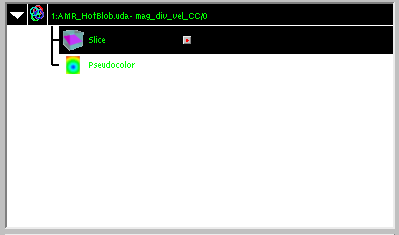
\includegraphics[width=0.8\textwidth]{VisItOrderOperator.png}
    \caption{Ordering of an operator and a plot}
    \label{VisItOrderOperator}
  \end{subfigure}
  \begin{subfigure}[b]{0.5\textwidth}
    \centering
    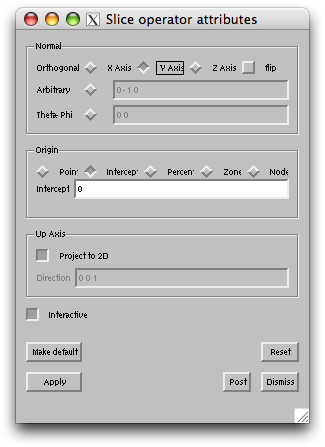
\includegraphics[height=0.2\textheight]{VisItSliceAtts.png}
    \caption{Slice plot attributes in \Visit}
    \label{VisItSliceAtts}
  \end{subfigure}
  \caption{Ordering and slicing.}
  \label{ucf:fig2}
\end{figure}

You can now play up with the various attributes (eg., selecting normal
plane) to obtain the desired visualization. The checkbox "Project to
2D" should be unchecked is you want to have the slice in 3D space.

\section{Vectors}
By default, \Visit reduces the number of vectors plotted (to 400) and
this needs to be manually changed to the original number or something
greater, only if required.  This can be accomplished by changing the
attributes of the Vector plot. In Figure~\ref{VisItVectorNumber}, the
number of vectors has been increased to 2000.
Also if you would like all the vectors to be visible, you would need
to switch off both the options, \Textsfc{Scale by magnitude} and
\Textsfc{Auto scale} under the Scale tab in the same window as
shown in figure~\ref{VisItVectorScale} describes this.

\begin{minipage}{\textwidth}
  \begin{minipage}{0.5\textwidth}
  \centering
  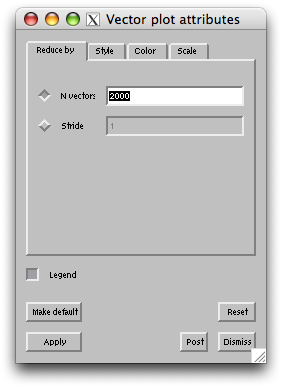
\includegraphics[height=0.2\textheight]{VisItVectorNumber.png}
  \captionof{figure}{Increasing the number of Vectors}
  \label{VisItVectorNumber}
  \end{minipage}
  \begin{minipage}{0.5\textwidth}
  \centering
  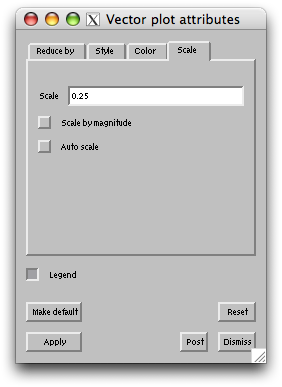
\includegraphics[height=0.2\textheight]{VisItVectorScale.png}
  \captionof{figure}{Increasing the scale of Vectors}
  \label{VisItVectorScale}
  \end{minipage}
\end{minipage}

\section{AMR datasets}
AMR datasets are read the same way as single level datasets. Once you
have it read, you can apply an plot/ operator on it. Since the dataset
is organized as levels and patches, you now have the flexibility of
visualizing each of them independently or as in a group. To achieve
this (assuming that you have already selected a plot), click on the
Subset button either on the Active Plots window in the gui or on the
same option in the Controls menu. This is illustrated in
Figures~\ref{VisItSubsetIcon} and ~\ref{VisItSubsetWin}.
\begin{figure}
  \centering
  \begin{subfigure}[b]{0.4\textwidth}
    \centering
    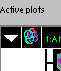
\includegraphics[height=0.2\textheight]{VisItSubsetIcon.png}
    \caption{Clicking on this icon opens the Subset window}
    \label{VisItSubsetIcon}
  \end{subfigure}
  \begin{subfigure}[b]{0.4\textwidth}
    \centering
    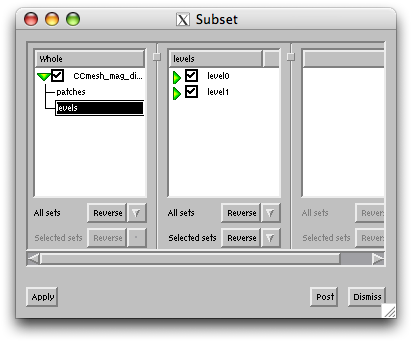
\includegraphics[height=0.2\textheight]{VisItSubsetWin.png}
    \caption{The Subset window in \Visit}
    \label{VisItSubsetWin}
  \end{subfigure}
  \caption{Visualizing AMR data}
  \label{ucf:fig3}
\end{figure}


\section{Examples}

\subsection{Volume visualization}

\begin{enumerate}

\item Read in the uda by selecting the index.xml file. A list of
  timesteps should now appear on the gui.


\item The first timestep (cycle 0000) should be preselected. In case you
are interested in plotting a different timestep, just double click on
it. Alternatively you can type it in the small rectangular box
(Figure~\ref{VisItTimestepBox}), just below the list of
timesteps. This can also be done at a later period in time, when you
are done plotting the variable associated with a specific timestep and
want to traverse through the others.


\item Next we select a variable to plotted. We click on the Plots
  menu, select the Volume plot and then select the variable tempIN as
  shown in the Figure~\ref{VisItVolumeTempINATK08}. The number '1'
  refers to the material associated with the variable.

\item The variable tempIN/1 now appears on the Active plots window
  (Figure~\ref{VisItDrawTempINATK08}). Select the variable and click
  Draw.

\begin{figure}[htb]
  \centering
  \begin{subfigure}[b]{0.3\textwidth}
    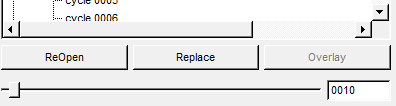
\includegraphics[width=0.9\textwidth]{VisItTimestepBox.png}
    \caption{The window on the gui lists all the timesteps}
    \label{VisItTimestepBox}
  \end{subfigure}
  \begin{subfigure}[b]{0.3\textwidth}
    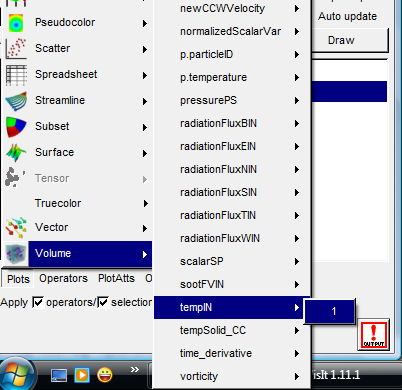
\includegraphics[width=0.9\textwidth]{VisItVolumeTempINATK08.png}
    \caption{Selecting a volume plot and an associated variable/ material}
    \label{VisItVolumeTempINATK08}
  \end{subfigure}
  \begin{subfigure}[b]{0.3\textwidth}
    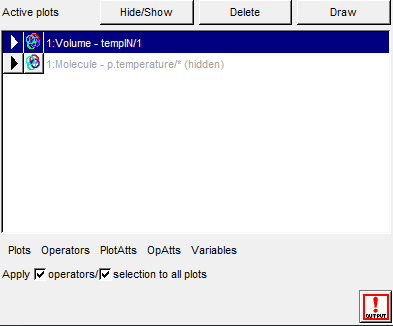
\includegraphics[width=0.9\textwidth]{VisItDrawTempINATK08.png}
    \caption{The list of plots in the Active plots window}
    \label{VisItDrawTempINATK08}
  \end{subfigure}
  \caption{}
  \label{ucf:fig4}
\end{figure}


\item A visualization now appears on the Viewer window, as shown in
  Figure~\ref{VisItVolumeTempINATK08Viewer}. You can interact with the
  visualization in terms of rotating it (holding the left mouse button
  and dragging it), zooming in/ out (scrolling the roller on the mouse
  and/ or selecting the magnifier at the top of the Viewer window)
  etc.


\item Once you have this basic volume visualization, you can change
  its attributes by double clicking on the Volume - tempIN/1 plot in
  the Active plots window. This pops up the Volume plot attributes
  window (Figure~\ref{VisItVolumeAttributes1} and
  figure~\ref{VisItVolumeAttributes2}).

\end{enumerate}


\begin{figure}[htb]
  \centering
  \begin{subfigure}[b]{0.3\textwidth}
    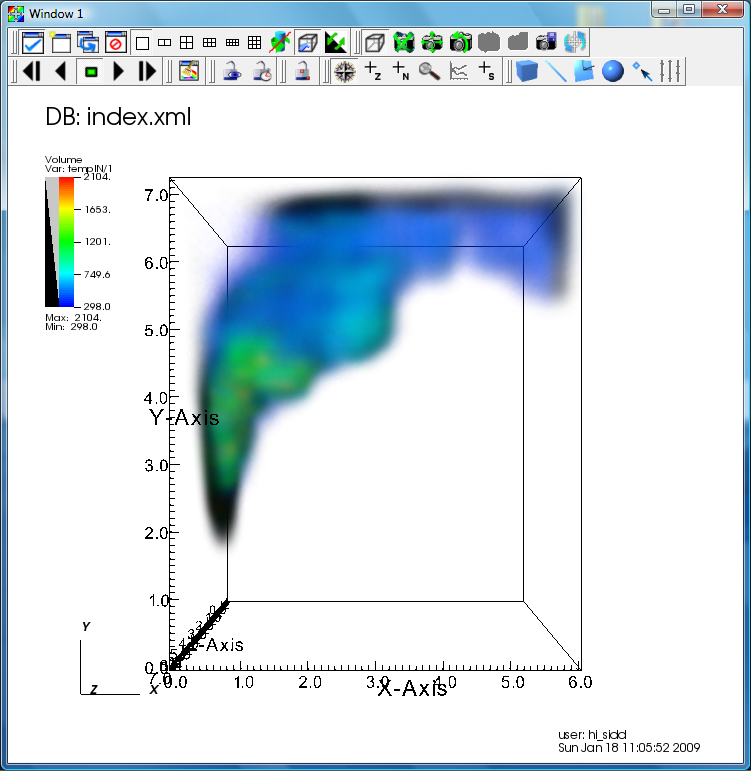
\includegraphics[width=0.9\textwidth]{VisItVolumeTempINATK08Viewer.png}
    \caption{Visualization of a volume on the viewer window}
    \label{VisItVolumeTempINATK08Viewer}
  \end{subfigure}
  \begin{subfigure}[b]{0.3\textwidth}
    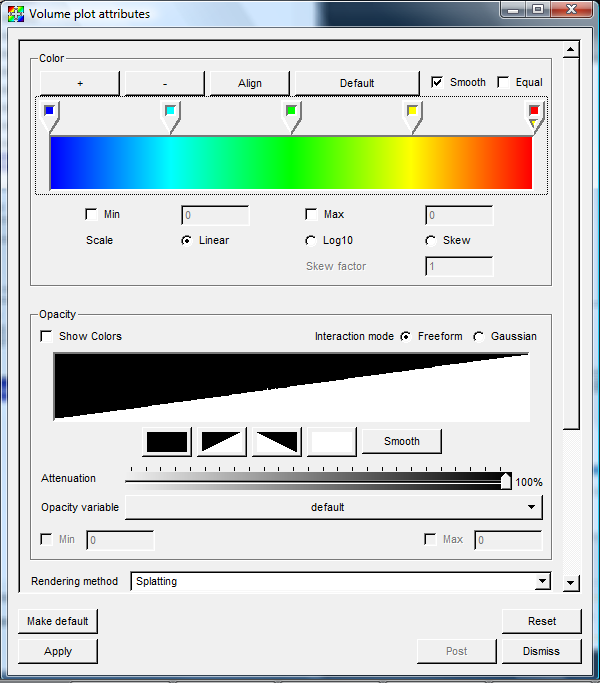
\includegraphics[width=0.9\textwidth]{VisItVolumeAttributes1.png}
    \caption{Volume visualization attributes window}
    \label{VisItVolumeAttributes1}
  \end{subfigure}
  \begin{subfigure}[b]{0.3\textwidth}
    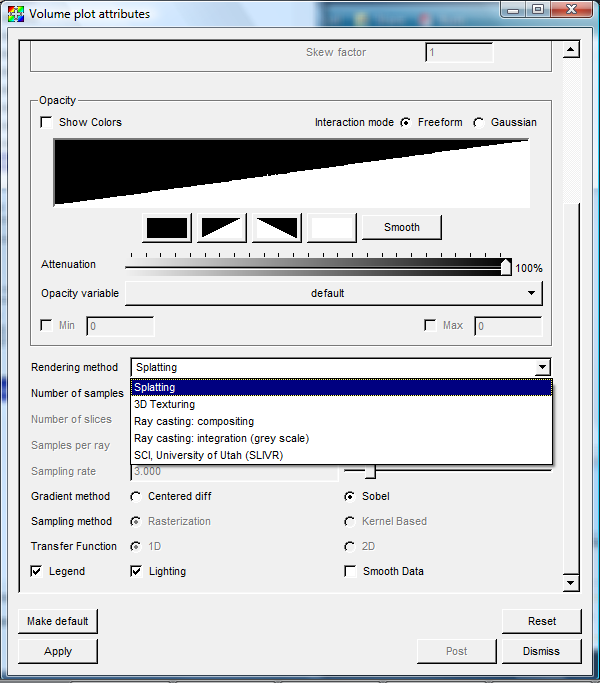
\includegraphics[width=0.9\textwidth]{VisItVolumeAttributes2.png}
    \caption{Volume visualization attributes window}
    \label{VisItVolumeAttributes2}
  \end{subfigure}
  \caption{}
  \label{ucf.fig5}
\end{figure}

The tab Color specifies the color table and the various options
associated with it. The user can add/ remove control points by
clicking on the + and - buttons. These can then be equally spaced by
pressing the Align button.

A different color table can be selected by clicking on the Default
button and then selecting an appropriate color table. The color(s)
associated with the control points can be changed by right-clicking on
the them and then selecting an appropriate color.

The user also has the option of specifying a Min and Max on the scalar
value range by checking on the associated box(s) and entering in the
values.

\begin{wrapfigure}{r}{.5\textwidth}
  \center
  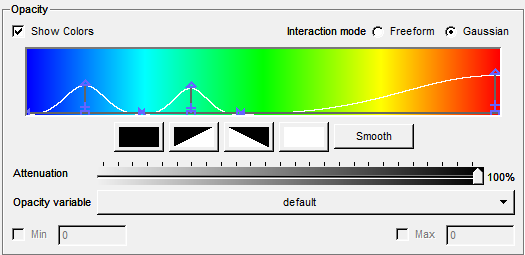
\includegraphics[width=.4\textwidth]{VisItTransferFunction.png}
  \caption{The opacity transfer function in the attributes window}
  \label{VisItTransferFunction}
\end{wrapfigure}

The second tab Opacity lets you specify a transfer function for the
color table. Clicking on the check box Show Colors copies the colors
from the color table onto this graph. Selecting the Interaction Mode
as Gaussian lets you draw curves and specify a more accurate color
table (Figure~\ref{VisItTransferFunction}).

You can add in as many curves on the graph by clicking on the left
mouse button and then placing them accordingly. To delete an unwanted
curve, just right click on it.

After specifying an opacity transfer function, one can select an
appropriate rendering method, Splatting being the default. The related
fields thereafter become active/ inactive as and when different
rendering methods are selected.

\subsection{Particle visualization}

\begin{enumerate}

\item To add particles, we select the Molecule plot and then click on
  the variable p.temperature as shown in the
  Figure~\ref{VisItMoleculePTempATK08}. The asterisk '*' refers to all
  the materials associated with the variable.


\item The variable p.temperature/* now appears on the Active plots
  list. Select the variable and hit Draw. A container in the form of
  particles now appears on the Viewer window.

\item Now double click on the variable name in Active plots list. This
  brings up the Molecule plot attributes window as shown in
  Figure~\ref{VisItMoleculeAttributesPTemp1}.

\end{enumerate}


\begin{figure}[htb]
  \centering
  \begin{subfigure}[b]{0.3\textwidth}
    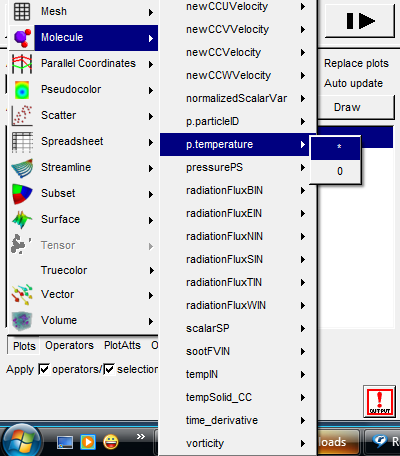
\includegraphics[width=0.9\textwidth]{VisItMoleculePTempATK08.png}
    \caption{Selecting a molecule plot and an associated variable/ material}
    \label{VisItMoleculePTempATK08}
  \end{subfigure}
  \begin{subfigure}[b]{0.3\textwidth}
    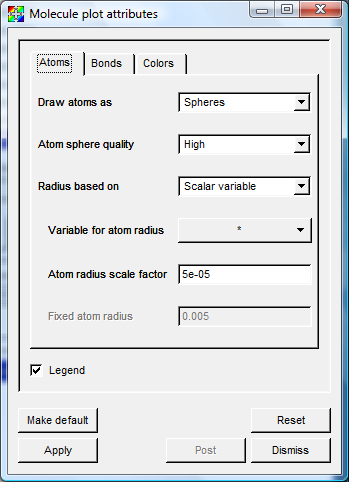
\includegraphics[width=0.9\textwidth]{VisItMoleculeAttributesPTemp1.png}
    \caption{Selecting a molecule plot and an associated variable/ material}
    \label{VisItMoleculeAttributesPTemp1}
  \end{subfigure}
  \begin{subfigure}[b]{0.3\textwidth}
    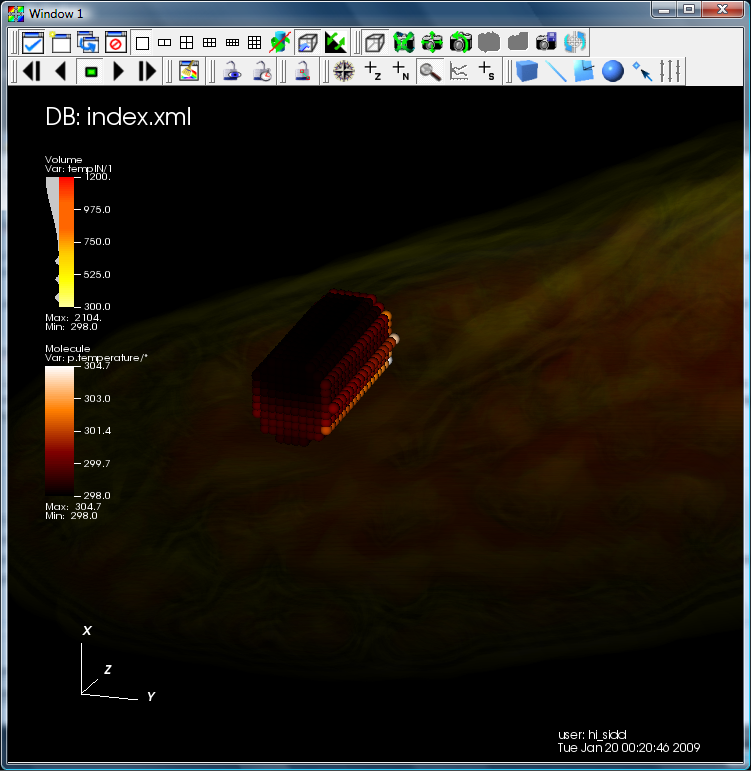
\includegraphics[width=0.9\textwidth]{VisItMoleculePTtempViewer.png}
    \caption{Selecting a molecule plot and an associated variable/ material}
    \label{VisItMoleculePTtempViewer}
  \end{subfigure}
  \caption{}
  \label{ucf.fig6}
\end{figure}

We choose to visualize the particles as Sphere Impostors (doesn't runs
the GPU out of memory, drawing as Spheres does). We also choose to
scale the sphere radius by a Scalar Variable and specify that variable
to be p.temperature/* itself (therefore the * appears). Since the
temperature values are too high, we scale them all by a factor of
5.e-05 (on the basis of trial and error). Finally in Colors tab, we
set the Color map for scalars as orangehot.  Combined with volume
visualization, we get a visualization as shown in
Figure~\ref{VisItMoleculePTtempViewer}.


\subsection{Visualizing patch boundaries}
In order to visualize patch boundaries, we use the Subset plot. As
with other variables, we select the Subset plot and an associated
variable. The variables have a prefix 'level/ patch'. There is a
level/ patch variable associated with every kind of variable (Cell
Centered, Node Centered, Face Centered) present in the dataset. In the
Figure~\ref{VisItSubsetPlotVariables}, we select one such variable.
Next, we hit Draw. This produces a visualization as shown in
Figure~\ref{VisItSubsetPlotViewer}.
\begin{figure}[htb]
  \centering
  \begin{subfigure}[b]{0.4\textwidth}
    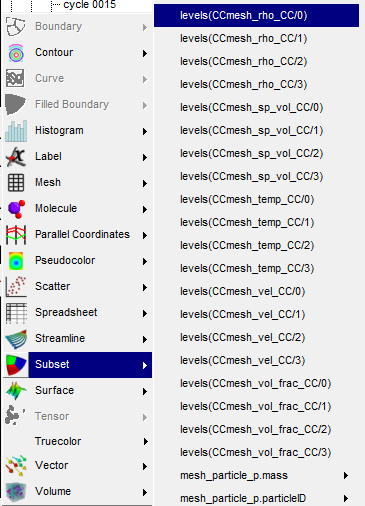
\includegraphics[width=0.8\textwidth]{VisItSubsetPlotVariables.png}
    \caption{A patch/ level variable, associated with every kind of variable}
    \label{VisItSubsetPlotVariables}
  \end{subfigure}
  \hspace{50pt}
  \begin{subfigure}[b]{0.4\textwidth}
    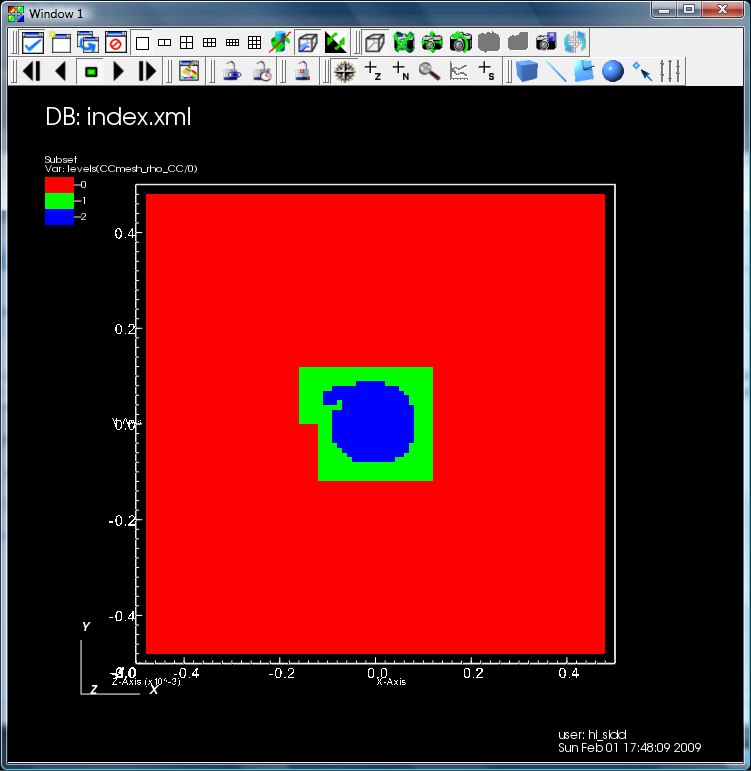
\includegraphics[width=0.8\textwidth]{VisItSubsetPlotViewer.png}
    \caption{The default visualization of patches}
    \label{VisItSubsetPlotViewer}
  \end{subfigure}
  \caption{}
  \label{ucf.fig7}
\end{figure}

To generate a wire-frame model, we double click on the Subset plot in
the Active plots window. This pops up the Subset plot attributes
window, where we check the Wireframe mode as shown in
Figure`\ref{VisItSubsetPlotAttrib}. This would produce a
visualization, similar to one shown in
Figure~\ref{VisItSubsetPlotWireframe}.
\begin{figure}[htb]
  \centering
  \begin{subfigure}[b]{0.4\textwidth}
    \centering
    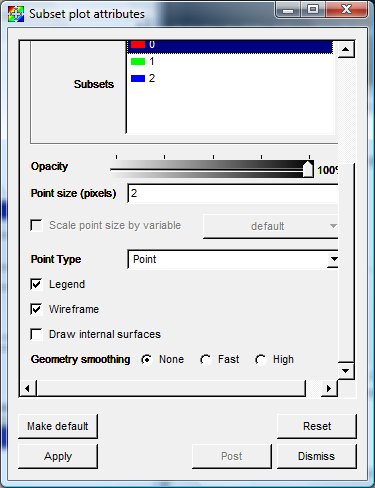
\includegraphics[width=0.8\textwidth]{VisItSubsetPlotAttrib.png}
    \caption{Enabling the 'Wireframe' mode for visualizing patch boundaries}
    \label{VisItSubsetPlotAttrib}
  \end{subfigure}
  \hspace{50pt}
  \begin{subfigure}[b]{0.4\textwidth}
    \centering
    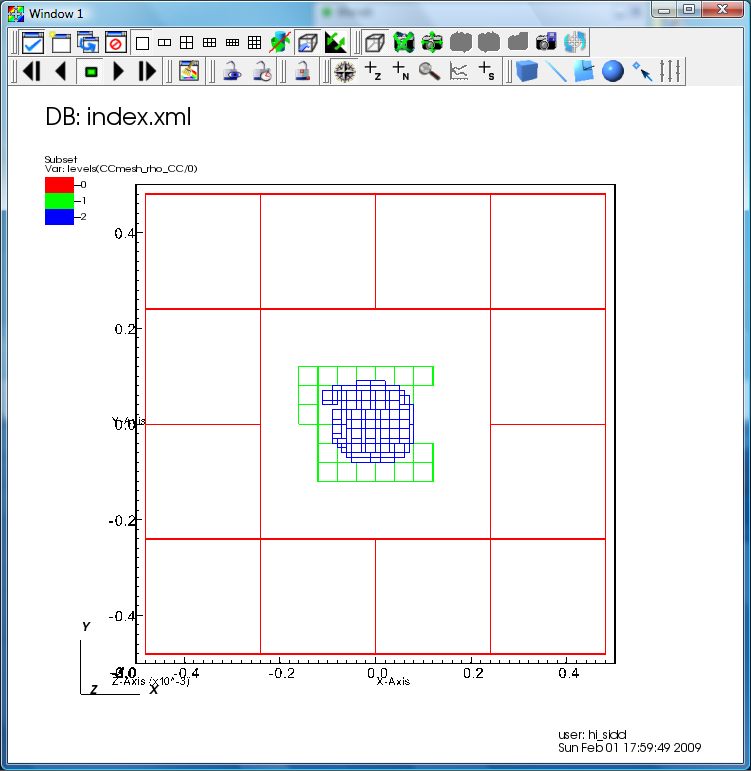
\includegraphics[width=0.8\textwidth]{VisItSubsetPlotWireframe.png}
    \caption{The patch boundaries after enabling the wireframe mode}
    \label{VisItSubsetPlotWireframe}
  \end{subfigure}
  \caption{}
  \label{ucf.fig8}
\end{figure}

\subsection{Iso-surfaces}

\begin{wrapfigure}[10]{r}{.5\textwidth}
  \vspace{-20pt}
  \centering
  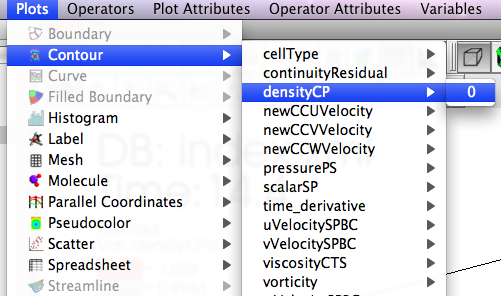
\includegraphics[width=0.4\textwidth]{VisItContourPlot.png}
  \caption{Selecting the 'Contour' plot on a regular 3D scalar variable}
  \label{VisItContourPlot}
\end{wrapfigure}

The easiest way to draw iso-surfaces is to use the 'Contour' Plot. As
with other plots demonstrated above, the contour plot is selected on a
regular 3D scalar variable. Figure ~\ref{VisItContourPlot} illustrates
this.

Once the plot is selected, we hit 'Draw'. This would produce a
visualization, similar to one shown in
Figure~\ref{VisItContourPlotViewer}. You can then modify the plot
attributes by double clicking on the plot in the 'Active plots'
window. This would pop up the 'Contour plot attributes window', as
shown in Figure~\ref{VisItContourPlotAttrib}.

The 'Select by' option can be changed to 'Value(s)' and
'Percent(s)'. When specifying multiple values, they should be
separated by a space.

\begin{figure}[htb]
  \centering
  \begin{subfigure}[b]{0.45\textwidth}
    \centering
    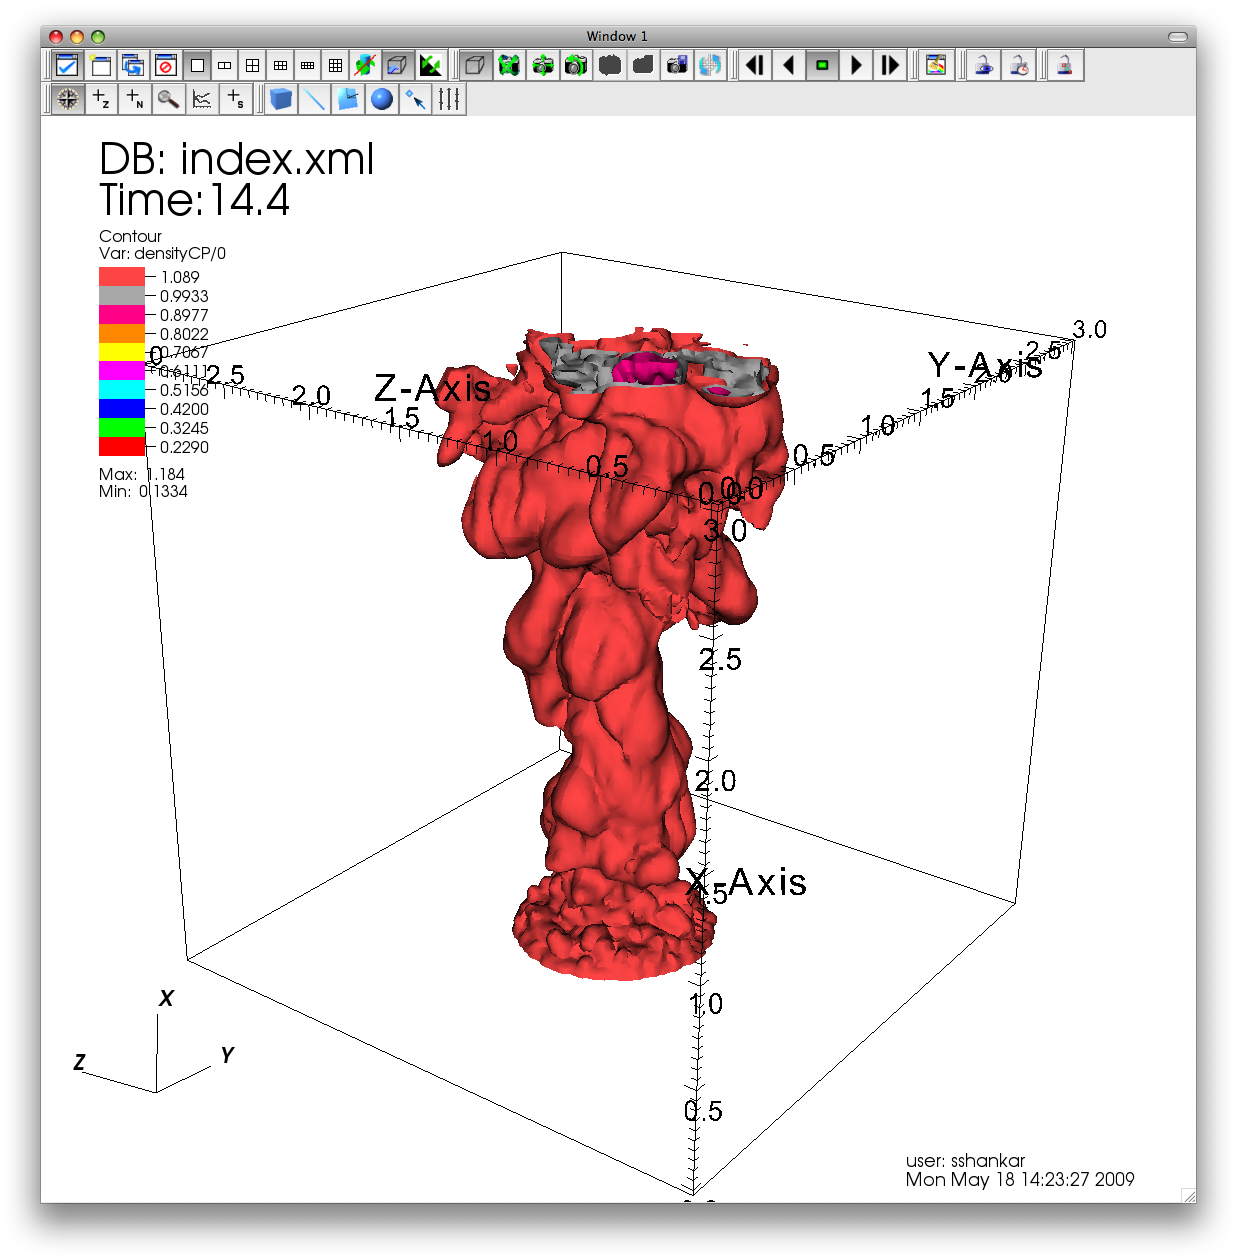
\includegraphics[height=0.15\textheight]{VisItContourPlotViewer.png}
    \caption{Iso-surface visualization}
    \label{VisItContourPlotViewer}
  \end{subfigure}
  \begin{subfigure}[b]{0.45\textwidth}
    \centering
    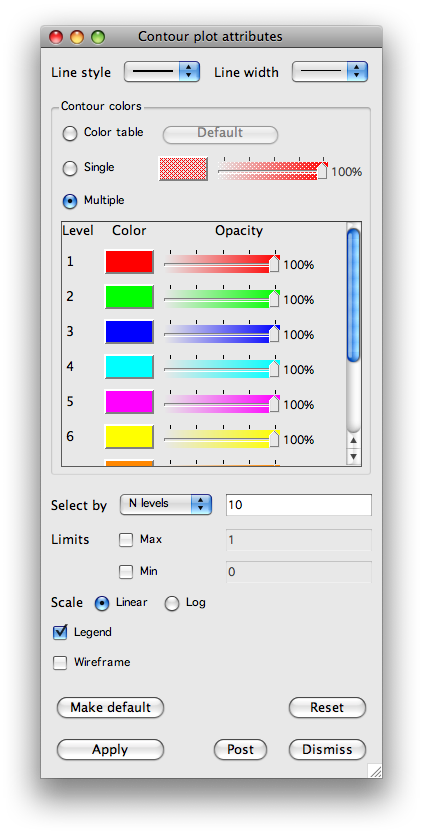
\includegraphics[height=0.15\textheight]{VisItContourPlotAttrib.png}
    \caption{The attributes window for the 'Contour' plot}
    \label{VisItContourPlotAttrib}
  \end{subfigure}
  \caption{}
  \label{ucf.fig9}
\end{figure}

\clearpage

\subsection{Streamlines}

\begin{wrapfigure}[9]{r}{.5\textwidth}
  \vspace{-20pt}
  \centering
  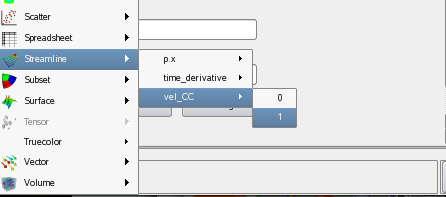
\includegraphics[width=.4\textwidth]{VisItStreamlinesPlot.png}
  \caption{Selecting the 'Streamlines' plot on a vector variable}
  \label{VisItStreamlinesPlot}
\end{wrapfigure}

As shown in Figure~\ref{VisItStreamlinesPlot} we select the
'Streamlines' plot on a vector variable. We then double click on the
plot itself, which pops up the 'Streamlines attributes window'.

We set the 'Distance' parameter such that it covers the entire
computational domain. We set the 'Streamline direction' as forward. In
the 'Source' tab, Figure~\ref{VisItStreamlinesAttrib1}, we define the
'Source type' as 'Line'. We can select other options too, notably
'Single Point', 'Sphere' etc. We now define the line 'Start' and 'End'
coordinates. In this specific case, we define them as [-0.1 -0.05 0]
and [-0.1 0.05 0] respectively. This choice ensures that we cover the
entire y axis and start at the leftmost corner of the computational
domain.

To ensure that our stream lines are smooth, we change the 'Maximum
step length' in the in the 'Advanced' tab. In this case, we change it
to 1.e-05. The thing to keep in mind is that this length should be
order of magnitude smaller than the length of the computational
domain. This is shown in Figure ~\ref{VisItStreamlinesAttrib2}.


Once these parameters are set, we hit 'Apply' and then click on the 'Draw' button on the gui. This produces a visualization similar to one shown in Figure ~\ref{VisItStreamlinesViewer}.
\begin{figure}[htb]
  \centering
  \begin{subfigure}[b]{0.3\textwidth}
  \centering
    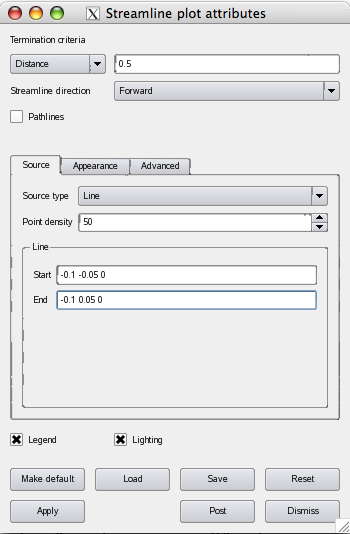
\includegraphics[width=0.9\textwidth]{VisItStreamlinesAttrib1.png}
    \caption{Setting the 'Source' tab parameters}
    \label{VisItStreamlinesAttrib1}
  \end{subfigure}
  \begin{subfigure}[b]{0.3\textwidth}
  \centering
    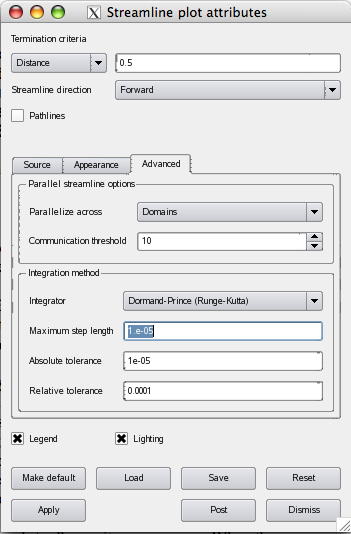
\includegraphics[width=0.9\textwidth]{VisItStreamlinesAttrib2.png}
    \caption{Setting the 'Advanced' tab parameters}
    \label{VisItStreamlinesAttrib2}
  \end{subfigure}
  \begin{subfigure}[b]{0.3\textwidth}
  \centering
    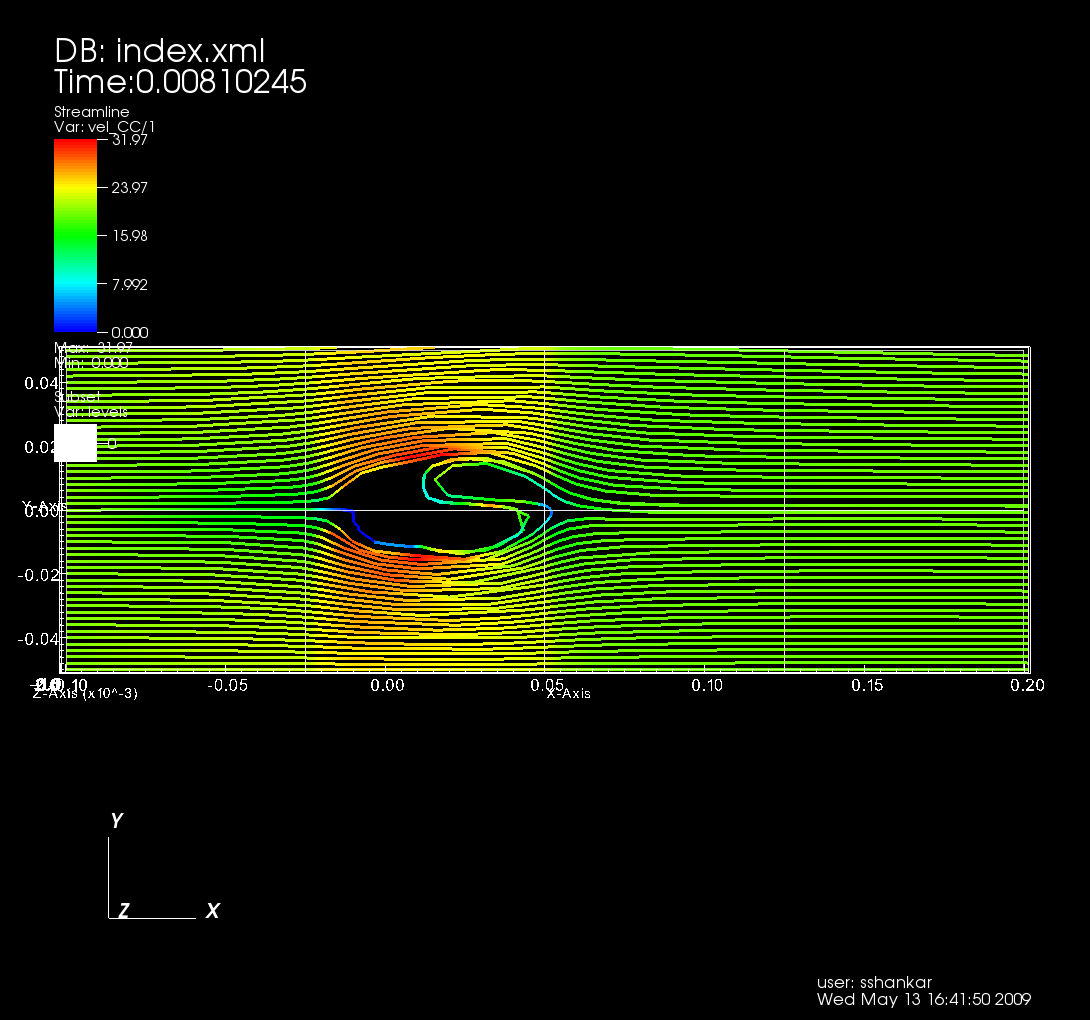
\includegraphics[width=0.9\textwidth]{VisItStreamlinesViewer.png}
    \caption{Streamlines visualization}
    \label{VisItStreamlinesViewer}
  \end{subfigure}
  \caption{}
  \label{ucf.fig10}
\end{figure}


\subsection{Visualizing extra cells}
For visualizing extra cells we use the 'Inverse Ghost Zone' operator
~\ref{VisItInverseGhostZoneOp} in conjunction with the 'Pseudocolor'
plot. Since the plugin reads in extra cells as ghost cells, the usage
of this operator make sense in this scenario.

After the operator is applied to the 'Pseudocolor' plot, we double
click on the operator to change its attributes. We switch to 'Both
ghost zones and real zones' in this window
~\ref{VisItInverseGhostZoneAttribs} and hit 'Apply'.

We then hit 'Draw'. When combined with the 'Mesh' plot we get a visualization similar to the one shown in Figure ~\ref{VisItInverseGhostZoneViewer}. The pick operations on the viewer can then be used to investigate the value(s) in these extra cells. 

\begin{figure}[htb]
  \centering
  \begin{subfigure}[b]{0.3\textwidth}
  \centering
    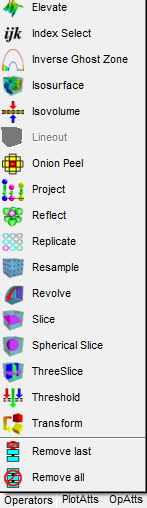
\includegraphics[height=0.3\textheight]{VisItInverseGhostZoneOp.png}
    \caption{Selecting the Inverse Ghost Zone operator}
    \label{VisItInverseGhostZoneOp}
  \end{subfigure}
  \begin{subfigure}[b]{0.3\textwidth}
  \centering
    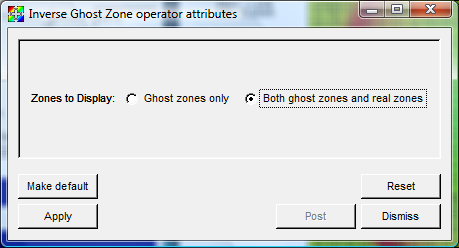
\includegraphics[width=0.9\textwidth]{VisItInverseGhostZoneAttribs.png}
    \caption{The attributes window for the 'Inverse Ghost Zone' operator}
    \label{VisItInverseGhostZoneAttribs}
  \end{subfigure}
  \begin{subfigure}[b]{0.3\textwidth}
  \centering
    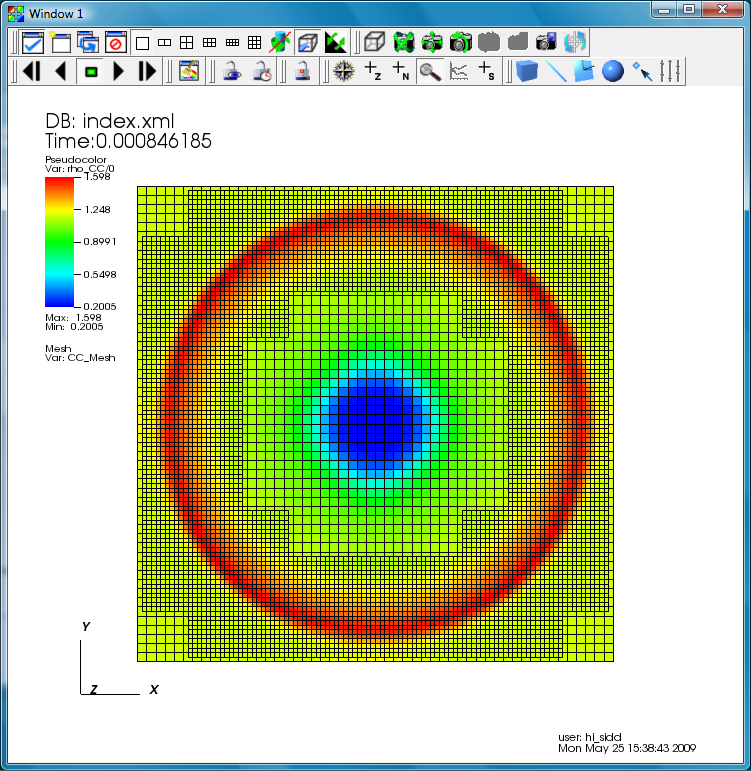
\includegraphics[width=0.9\textwidth]{VisItInverseGhostZoneViewer.png}
    \caption{Extra cells together with the 'Mesh' plot}
    \label{VisItInverseGhostZoneViewer}
  \end{subfigure}
  \caption{}
  \label{ucf.fig11}
\end{figure}


\subsection{Picking on particles}

 \begin{wrapfigure}[4]{r}{.5\textwidth}
   \vspace{-40pt}
   \center
   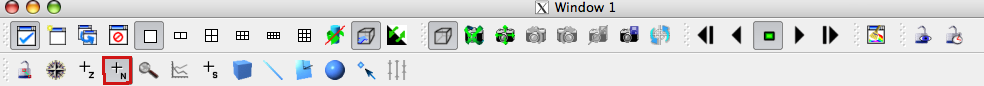
\includegraphics[width=0.5\textwidth]{VisItNodePick.png}
   \caption{The 'Node pick mode' on the visualization window}
   \label{VisItNodePick}
 \end{wrapfigure}

The 'Node pick mode' on the visualization window can be used to pick
particles and investigate particles attributes. After plotting
particles using the 'Molecule' plot, the user can then select the
'Node pick mode' ~\ref{VisItNodePick} and select particles (by
clicking on them) of interest.

 \begin{wrapfigure}[10]{r}{.5\textwidth}
   \vspace{-20pt}
  \centering
  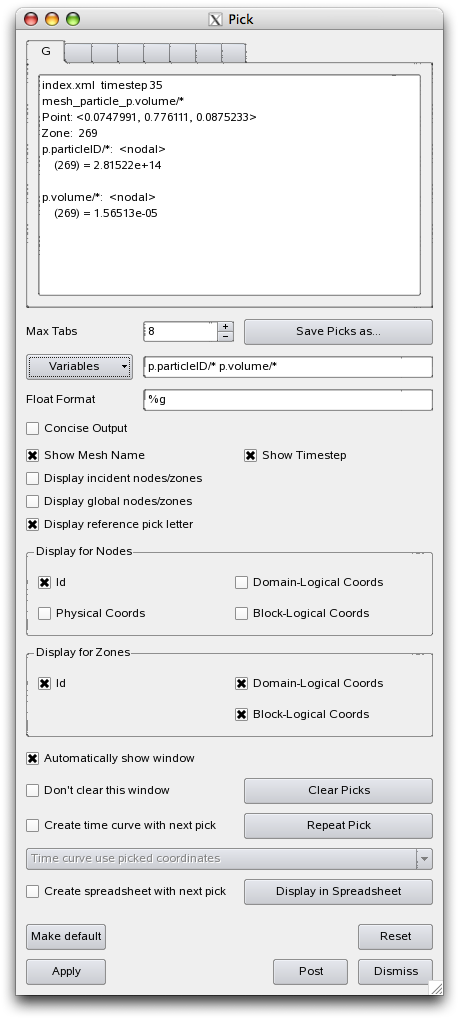
\includegraphics[height=0.2\textheight]{VisItPickWindow.png}
  \caption{The 'Pick' window}
  \label{VisItPickWindow}
\end{wrapfigure}

Once a particle is picked, the 'Pick' window pops up with the particle
attributes. By default only the variable plotted is queried, if the
user wants to query more variables per pick - they can be added by
selecting additional variables from the 'Variables' menu and as shown
in the Figure ~\ref{VisItPickWindow}.


\subsection{Selectively visualizing vectors}
The expression editor can be used to define a vector variable with magnitude greater or lesser than a certain extent. An example of this is shown below,
\begin{lstlisting}[backgroundcolor=\color{background}]
if(gt(magnitude(<vel_CC/1>), 0.0), <vel_CC/1>, {0, 0, 0})
\end{lstlisting}

Put into words, if magnitude of \lstinline!vel_CC/1! is greater than 0.0, display it, else display a zero magnitude vector. To use the 'lesser than' parameter, replace 'gt' with 'lt'.


